\documentclass[aspectratio=169,11pt]{beamer}

% common_setting.tex
% Shared preamble for the five PSPDE2026 workshop beamer decks (00-04).
% \input this right after \documentclass in each deck.
% Requires xelatex (fontspec/unicode-math need XeTeX or LuaTeX, not pdflatex).

% Fonts
\usepackage{fontspec}
\usepackage{unicode-math}
\setmainfont{Liberation Sans}
\setsansfont{Liberation Sans}
\setmonofont{Liberation Mono}[Scale=0.85]
\setmathfont{Latin Modern Math}

% Theme and colors
\usetheme{moloch}
\molochset{
  block=fill,
  progressbar=frametitle,
  sectionpage=progressbar,
}
\setbeamertemplate{page number in head/foot}[totalframenumber]

% Graphics
\usepackage{graphicx}
\graphicspath{{./figures/}}

% Tables
\usepackage{booktabs}
\usepackage{tabularx}

% Unnumbered captions without the "Figure:" label prefix
\usepackage{caption}
\captionsetup{labelformat=empty}

% Code listings
\usepackage{listings}
\usepackage{xcolor}
\definecolor{codebg}{RGB}{245,245,245}
% moloch's own accent colors, aliased under their original Metropolis names
\colorlet{mAlertFg}{mLightBrown}
\colorlet{mExampleFg}{mLightGreen}
\lstdefinestyle{python}{
  language=Python,
  basicstyle=\ttfamily\scriptsize,
  keywordstyle=\color{mAlertFg}\bfseries,
  commentstyle=\color{mExampleFg}\itshape,
  stringstyle=\color{mExampleFg!70!black},
  backgroundcolor=\color{codebg},
  rulecolor=\color{black!15},
  frame=single,
  breaklines=true,
  showstringspaces=false,
  columns=fullflexible,
  numbers=none
}
\lstdefinestyle{shell}{
  basicstyle=\ttfamily\scriptsize,
  backgroundcolor=\color{codebg},
  rulecolor=\color{black!15},
  frame=single,
  breaklines=true,
  columns=fullflexible
}


% Title information
\title[apsg basics]{Structural Geology with \texttt{apsg}}
\subtitle{Block 1 --- Modern Workflow in Geology}
\author[O.\ Lexa]{Ondrej Lexa}
\institute[Charles University]{
  Institute of Petrology and Structural Geology (IPSG)\\
  Charles University, Prague, Czechia
}
\date{8 October 2026}

\begin{document}

\begin{frame}[plain]
  \titlepage
\end{frame}

\section{Motivation}

\begin{frame}{This Block (9:30--11:00)}
  \begin{block}{Objective}
    Manipulate, analyse and project orientation data --- the things structural
    geologists need every day --- in a few lines of reproducible code.
  \end{block}
  \vspace{0.3cm}
  \begin{enumerate}
    \item Basic objects: \texttt{vec}, \texttt{lin}, \texttt{fol}, \texttt{pair}, \texttt{fault}
    \item Feature sets and field data from CSV
    \item Stereonets: points, great circles, density contours
    \item Population analysis: mean, Fisher statistics, eigenvectors, fold axes
    \item Saving vector graphics for publication
  \end{enumerate}
  \vspace{0.2cm}
  \small Notebook: \texttt{notebooks/01\_apsg\_basics.ipynb}
\end{frame}

\begin{frame}{Why Objects?}
  \begin{columns}[T]
    \begin{column}{0.48\textwidth}
      \begin{alertblock}{Two numbers in a spreadsheet}
        \small
        \texttt{120, 60} --- a lineation? a plane? dip direction or strike?
        Every calculation (poles, intersections, rotations, means) has to
        re-encode that meaning by hand.
      \end{alertblock}
    \end{column}
    \begin{column}{0.48\textwidth}
      \begin{exampleblock}{An \texttt{apsg} object}
        \small
        \texttt{fol(120, 60)} \emph{is} a plane. It knows its pole, how to
        intersect with another plane, how to rotate, how to plot itself, and
        what its mean with other planes means.
      \end{exampleblock}
    \end{column}
  \end{columns}
  \vspace{0.4cm}
  \begin{block}{apsg in one sentence}
    A Python package for structural geologists: orientation \textbf{features},
    \textbf{sets} of features, \textbf{tensors}, and \textbf{plots} that
    understand them.
  \end{block}
\end{frame}

\section{Basic Objects}

\begin{frame}[fragile]{Vectors}
  \begin{columns}[T]
    \begin{column}{0.55\textwidth}
      \begin{lstlisting}[style=python]
from apsg import *

u = vec(1, -2, 3)     # components
v = vec(120, 60)      # azimuth, inclination

abs(u)                # length
u + v                 # sum
u @ v                 # dot product
u.cross(v)            # cross product
u.angle(v)            # angle in degrees
u.rotate(v, 45)       # rotate u around v
      \end{lstlisting}
    \end{column}
    \begin{column}{0.42\textwidth}
      \small
      \begin{itemize}
        \item Geographic frame: $x$ = north, $y$ = east, $z$ = down
        \item Ordinary vector algebra with Python operators
        \item The foundation for every other feature type
      \end{itemize}
    \end{column}
  \end{columns}
\end{frame}

\begin{frame}[fragile]{Lineations and Foliations}
  \begin{columns}[T]
    \begin{column}{0.55\textwidth}
      \begin{lstlisting}[style=python]
l = lin(120, 60)       # trend / plunge
f = fol(216, 62)       # dip direction / dip

fol("N30E,40NW")       # quadrant notation
with apsg_conf_context(notation="rhr"):
    print(f)           # S:126/62  (strike RHR)

lin(f)                 # pole to the plane
fol(l)                 # plane normal to line
lin(f.dipvec())        # dip vector
lin(f.rake(30))        # line with rake 30
      \end{lstlisting}
    \end{column}
    \begin{column}{0.42\textwidth}
      \small
      \begin{itemize}
        \item \texttt{lin} and \texttt{fol} are \textbf{axial} and always lower hemisphere
        \item A foliation is stored by its \textbf{pole}
        \item Input and output notation is configurable
              (\texttt{dd}, \texttt{rhr}, \texttt{quadrant})
        \item Conversions are explicit: \texttt{lin(f)}, \texttt{fol(l)}
      \end{itemize}
    \end{column}
  \end{columns}
\end{frame}

\begin{frame}[fragile]{The Geological Cross Product}
  \begin{columns}[T]
    \begin{column}{0.55\textwidth}
      \begin{lstlisting}[style=python]
f1, f2 = fol(250, 40), fol(160, 30)

f1 ** f2            # intersection: L:195/25
lin(250, 40) ** lin(160, 30)
                    # plane through both lines
f1.angle(f2)        # 48.4 deg

s = StereoNet()
s.great_circle(f1, f2, label="planes")
s.pole(f1, f2, color="k", label="poles")
s.line(f1 ** f2, color="r", ms=8)
s.show()
      \end{lstlisting}
    \end{column}
    \begin{column}{0.42\textwidth}
      \begin{figure}
        \centering
        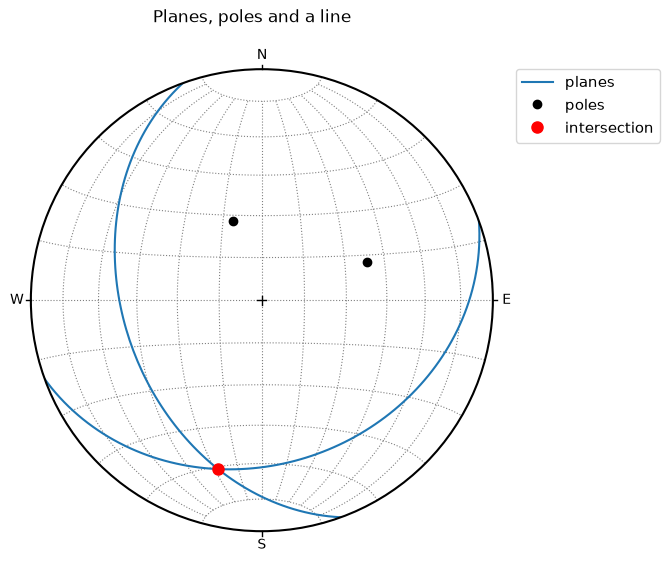
\includegraphics[width=\textwidth,height=0.7\textheight,keepaspectratio]{nb_planes_poles.png}
      \end{figure}
    \end{column}
  \end{columns}
\end{frame}

\begin{frame}[fragile]{Pairs and Faults}
  \begin{lstlisting}[style=python]
p = pair(120, 40, 162, 28)        # plane + line in it (e.g. S + stretching L)
p.misfit                          # 3.56 deg: measured line not exactly in plane
p.fol, p.lin, p.rake              # adjusted, perfectly orthogonal pair

ft = fault(120, 60, 110, 58, "n") # pair + sense of movement
ft.p, ft.t, ft.m                  # P axis, T axis, movement plane
fault(140, 30, 110, 26, "r")      # sense: 1/"n", -1/"r", "s", "d"
fault(fol(120, 80), lin(32, 10), "s")
  \end{lstlisting}
  \vspace{0.2cm}
  \small
  \begin{itemize}
    \item Real measurements never fit perfectly --- \texttt{pair} corrects them
          symmetrically and reports the misfit
    \item \texttt{fault} is the starting point for kinematic and stress analysis (Block 2)
  \end{itemize}
\end{frame}

\section{Feature Sets \& Stereonets}

\begin{frame}[fragile]{Feature Sets}
  \begin{lstlisting}[style=python]
L = G([lin(120, 60), lin(116, 50), lin(132, 45), lin(90, 60)])  # -> LineationSet
L[0], len(L), L[1:3]              # behaves like a list

cluster = linset.random_fisher(position=lin(120, 40), kappa=30, n=100)
S = folset.from_csv("planes.csv", acol="azi", icol="inc")
  \end{lstlisting}
  \vspace{0.2cm}
  \begin{center}
    \small
    \begin{tabular}{ll}
      \toprule
      \textbf{Single feature} & \textbf{Set} \\
      \midrule
      \texttt{vec}, \texttt{lin}, \texttt{fol} & \texttt{vecset}, \texttt{linset}, \texttt{folset} \\
      \texttt{pair}, \texttt{fault} & \texttt{pairset}, \texttt{faultset} \\
      any list of features & \texttt{G([...])} picks the right set type \\
      \bottomrule
    \end{tabular}
  \end{center}
  \small Sets add group methods: mean, statistics, orientation tensor, rotation, \ldots
\end{frame}

\begin{frame}[fragile]{Stereonets}
  \begin{columns}[T]
    \begin{column}{0.55\textwidth}
      \begin{lstlisting}[style=python]
s = StereoNet(title="Density contours")
s.contour(cluster, levels=8, colorbar=True)
s.line(cluster, color="k", ms=3)
s.confidence(cluster, method="fisher",
             level=0.95, color="r")
s.show()
      \end{lstlisting}
      \vspace{0.1cm}
      \footnotesize
      \begin{tabular}{ll}
        \toprule
        \texttt{s.line / s.pole} & points \\
        \texttt{s.great\_circle} & planes \\
        \texttt{s.contour} & density (Kamb) \\
        \texttt{s.confidence} & cone around mean \\
        \texttt{s.pair / s.fault} & composite features \\
        \bottomrule
      \end{tabular}
    \end{column}
    \begin{column}{0.42\textwidth}
      \begin{figure}
        \centering
        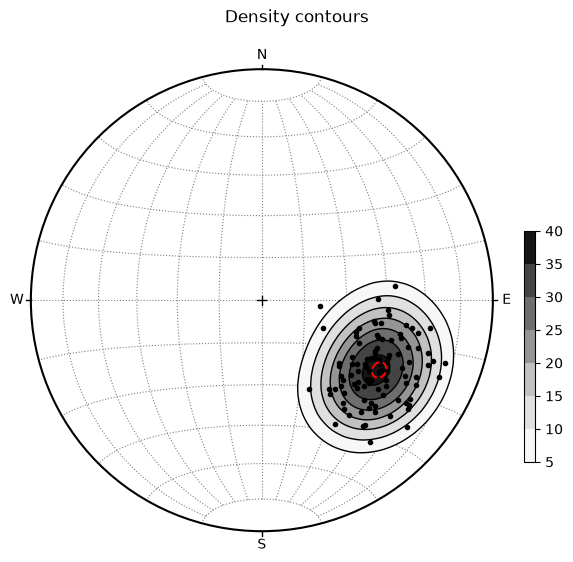
\includegraphics[width=\textwidth,height=0.75\textheight,keepaspectratio]{nb_contour_cluster.png}
      \end{figure}
    \end{column}
  \end{columns}
\end{frame}

\begin{frame}{Projection Options}
  \begin{columns}[T]
    \begin{column}{0.45\textwidth}
      \small
      \begin{itemize}
        \item \texttt{StereoNet()} --- equal-area (Schmidt), lower hemisphere
        \item \texttt{kind="equal-angle"} --- Wulff net
        \item \texttt{hemisphere="upper"}
        \item \texttt{grid=False}, \texttt{title=...}
        \item Global look via \texttt{apsg\_conf}, e.g.\ \texttt{apsg\_conf.figsize}
      \end{itemize}
    \end{column}
    \begin{column}{0.52\textwidth}
      \begin{figure}
        \centering
        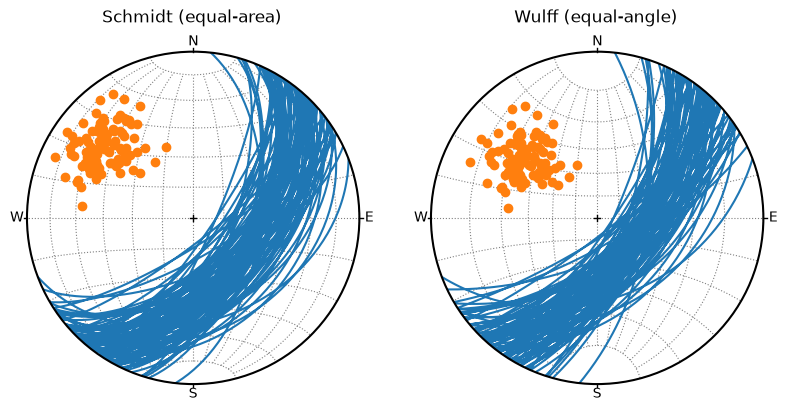
\includegraphics[width=\textwidth,height=0.65\textheight,keepaspectratio]{apsg_schmidt_wulff.png}
        \caption*{\footnotesize Schmidt vs.\ Wulff net (apsg docs)}
      \end{figure}
    \end{column}
  \end{columns}
\end{frame}

\section{Population Analysis}

\begin{frame}[fragile]{Mean Orientation and Fisher Statistics}
  \begin{columns}[T]
    \begin{column}{0.55\textwidth}
      \begin{lstlisting}[style=python]
cluster.R()                   # mean: L:121/41
st = cluster.fisher_statistics()
st["k"], st["alpha"]          # 31.0, 2.6 deg
cluster.var()                 # spherical variance
      \end{lstlisting}
      \small
      \begin{itemize}
        \item \texttt{R()} --- resultant (mean) direction
        \item \texttt{k} --- precision; \texttt{alpha} --- 95\,\% cone
        \item Also \texttt{bingham\_statistics}, \texttt{watson\_statistics},
              \texttt{bootstrap}
      \end{itemize}
    \end{column}
    \begin{column}{0.42\textwidth}
      \begin{figure}
        \centering
        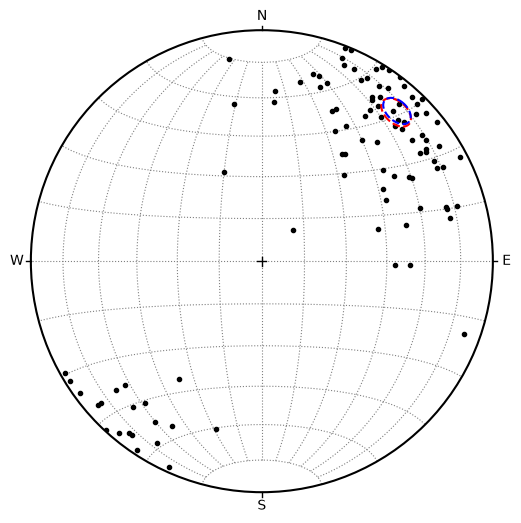
\includegraphics[width=\textwidth,height=0.65\textheight,keepaspectratio]{apsg_fisher_bootstrap.png}
        \caption*{\footnotesize Fisher vs.\ bootstrap cones (apsg docs)}
      \end{figure}
    \end{column}
  \end{columns}
\end{frame}

\begin{frame}[fragile]{Orientation Tensor and Eigenvectors}
  \begin{columns}[T]
    \begin{column}{0.55\textwidth}
      \begin{lstlisting}[style=python]
ot = girdle.ortensor()
ot.eigenvalues()   # [0.625 0.375 0.   ]
ot.eigenlins()     # principal axes
ot.eigenfols(2)    # best-fit girdle plane
ot.P, ot.G, ot.R   # point/girdle/random

s = StereoNet()
s.pole(girdle, ms=3)
s.line(*ot.eigenlins(), color="r", ms=8)
s.great_circle(ot.eigenfols(2), color="r")
      \end{lstlisting}
      \small Works for clusters \emph{and} girdles --- where a simple mean fails.
    \end{column}
    \begin{column}{0.42\textwidth}
      \begin{figure}
        \centering
        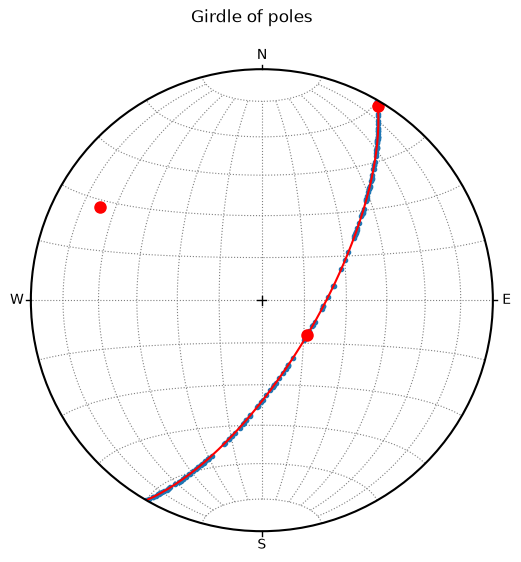
\includegraphics[width=\textwidth,height=0.72\textheight,keepaspectratio]{nb_girdle.png}
      \end{figure}
    \end{column}
  \end{columns}
\end{frame}

\begin{frame}[fragile]{Fold Axis from Folded Foliations}
  \begin{columns}[T]
    \begin{column}{0.5\textwidth}
      \begin{lstlisting}[style=python]
from apsg.pandas import pd
df = pd.read_csv("data/structures.csv")
S1 = df[df.structure == "S1"].fol(name="S1")
L3 = df[df.structure == "L3"].lin(name="L3")

beta = S1.ortensor().eigenlins(2)
# beta (S1 girdle axis): L:118/12
# mean L3              : L:122/8
      \end{lstlisting}
      \small
      Poles of a cylindrically folded surface lie on a $\pi$-girdle; the
      \textbf{smallest eigenvector} is the fold axis $\beta$. Here it matches the
      independently measured L3 within 6\textdegree.
    \end{column}
    \begin{column}{0.47\textwidth}
      \begin{figure}
        \centering
        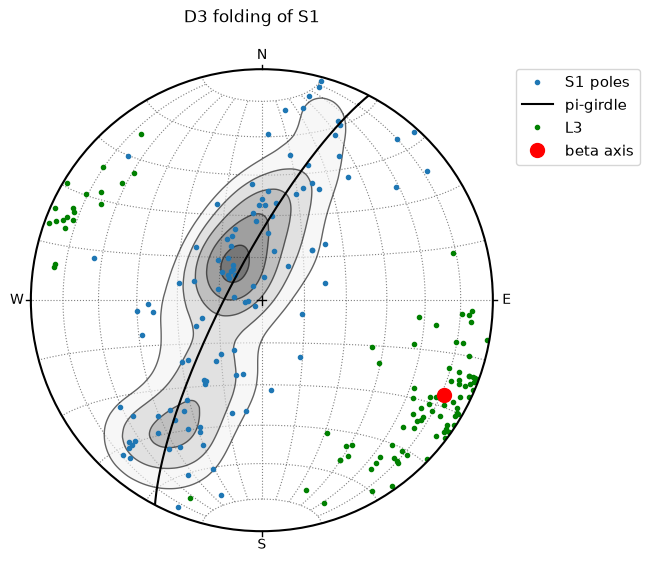
\includegraphics[width=\textwidth,height=0.75\textheight,keepaspectratio]{nb_beta_S1_L3.png}
      \end{figure}
    \end{column}
  \end{columns}
\end{frame}

\section{Field Data \& Output}

\begin{frame}[fragile]{Reading Field Data with pandas}
  \begin{lstlisting}[style=python]
from apsg.pandas import pd, gbf       # registers df.lin, df.fol, df.vec, df.fault

df = pd.read_csv("data/structures.csv")          # columns: site, structure, azi, inc
S1 = df[df.structure == "S1"].fol(name="S1")     # -> FoliationSet
df[df.structure == "L3"].lin.groupby("site").apply(gbf.mean)   # mean L3 per site
df[df.structure == "S1"].fol.plot(kind="pole")   # quick stereonet

wide = pd.read_csv("data/structures_wide.csv")   # S1_azi, S1_inc, L1_azi, ...
wide.fol.set_columns(azi="S1_azi", inc="S1_inc")
S1_wide = wide.fol(name="S1")                    # rows with missing values skipped
  \end{lstlisting}
  \vspace{0.1cm}
  \small Excel works the same: \texttt{pd.read\_excel("field.xlsx", sheet\_name="S1")}
\end{frame}

\begin{frame}[fragile]{Saving Vector Graphics}
  \begin{lstlisting}[style=python]
s = StereoNet(title="S1 and L3")
s.great_circle(S1, color="0.7", lw=0.5)
s.line(L3, color="g", ms=4, label="L3")
s.line(beta, color="r", ms=10, label="beta")
s.savefig("output/S1_L3.pdf")               # vector - edit in Inkscape/Illustrator
s.savefig("output/S1_L3.svg")               # vector
s.savefig("output/S1_L3.png", dpi=300)      # raster
  \end{lstlisting}
  \vspace{0.2cm}
  \small
  \begin{itemize}
    \item The file extension selects the format; all other keywords go to matplotlib
  \end{itemize}
\end{frame}

\section{Hands-on}

\begin{frame}{Hands-on Exercise}
  \begin{columns}[T]
    \begin{column}{0.55\textwidth}
      \small
      \textbf{\texttt{data/field\_measurements.csv}} --- bedding S0, cleavage S1
      and intersection lineation L1 from 12 stations
      \begin{enumerate}
        \item Load it; build sets for S0, S1, L1
        \item S0 poles with contours, S1 as great circles, L1 as points
        \item Fold axis $\beta$ from S0; compare with mean L1 --- does $\beta$
              lie in the mean S1 (axial-planar cleavage)?
        \item Mean S1 and its Fisher $\alpha_{95}$
        \item Save the stereonet as PDF and SVG
      \end{enumerate}
    \end{column}
    \begin{column}{0.42\textwidth}
      \begin{figure}
        \centering
        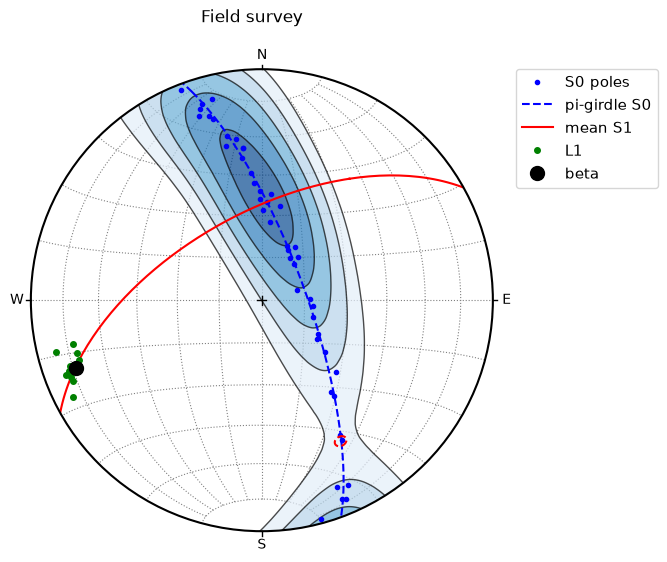
\includegraphics[width=\textwidth,height=0.7\textheight,keepaspectratio]{nb_field_survey.png}
        \caption*{\footnotesize Target result (solution in the notebook)}
      \end{figure}
    \end{column}
  \end{columns}
\end{frame}

\section{Recap}

\begin{frame}{Recap}
  \centering
  \small
  \begin{tabular}{ll}
    \toprule
    \textbf{Task} & \textbf{Code} \\
    \midrule
    Create features & \texttt{vec(1,2,3)}, \texttt{lin(120,60)}, \texttt{fol(216,62)}, \texttt{pair}, \texttt{fault} \\
    Convert & \texttt{lin(f)} (pole), \texttt{fol(l)}, \texttt{f1 ** f2} (intersection) \\
    Collections & \texttt{G([...])}, \texttt{linset}, \texttt{folset}, \texttt{df.fol()}, \texttt{df.lin()} \\
    Plot & \texttt{StereoNet()} $\rightarrow$ \texttt{line/pole/great\_circle/contour} $\rightarrow$ \texttt{savefig} \\
    Statistics & \texttt{.R()}, \texttt{.fisher\_statistics()}, \texttt{.ortensor().eigenlins()} \\
    Fold axis & \texttt{S.ortensor().eigenlins(2)} \\
    \bottomrule
  \end{tabular}

  \vspace{0.4cm}
  \raggedright
  \textbf{Resources:} \texttt{github.com/ondrolexa/apsg} --- docs with tutorial notebooks
  \vspace{0.3cm}

  \centering \Large Next: faults, tensors and stress inversion
\end{frame}

\end{document}
